\documentclass{beamer}
\usetheme{Copenhagen}
\usepackage{tikz}
\usepackage{multirow}
\usepackage{graphicx}
\usepackage{epstopdf}
\usepackage{subfigure}
\graphicspath{{img/}}

\title[How Data Centers Provide Consumer Services]{How Data Centers Provide Consumer Services}
\institute{}
\author{Original author: Tom Coughlin}
\date{November 2, 2017}

\begin{document}
  \begin{frame}
    \titlepage
  \end{frame}

  \section{Introduction}
  \begin{frame}{Introduction}{Why we need data centers}
    Mobile devices have the ability to store and process data, and we can do these locally. But
    \pause
    \begin{itemize}
      \item the storage capacity is very limited (usually less than 128 GB)
      \item the processing power is also limited
    \end{itemize}
    \pause
    So, we can transfer and store the data in a cloud server, process on the cloud server, and get back the result.
    \begin{figure}
        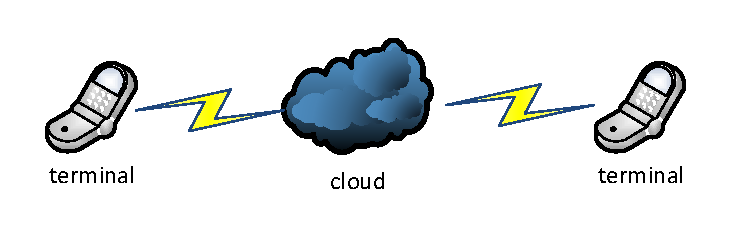
\includegraphics[width = 7cm]{topo1.pdf}
        \caption{Mobile devices depend upon cloud servers}
    \end{figure}
  \end{frame}

  \section{Content Delivery}
  \begin{frame}{Content Delivery}{Disadvantages of single content server}
    It is of low efficiency if all content is delivered from a central server (or cluster), especially for those users far from server:
    \begin{itemize}
      \item the high latency may lower user experience
      \item the cost of data transmission may be large
    \end{itemize}
    \pause
    We can use edge servers to help deliver the content, which are geographically distributed all over the world.
    Edge servers store copies of frequently visited content, while central server provide those that are less frequently visited.
  \end{frame}

  \begin{frame}{Content Delivery}{Content distribution system}
    \begin{figure}
        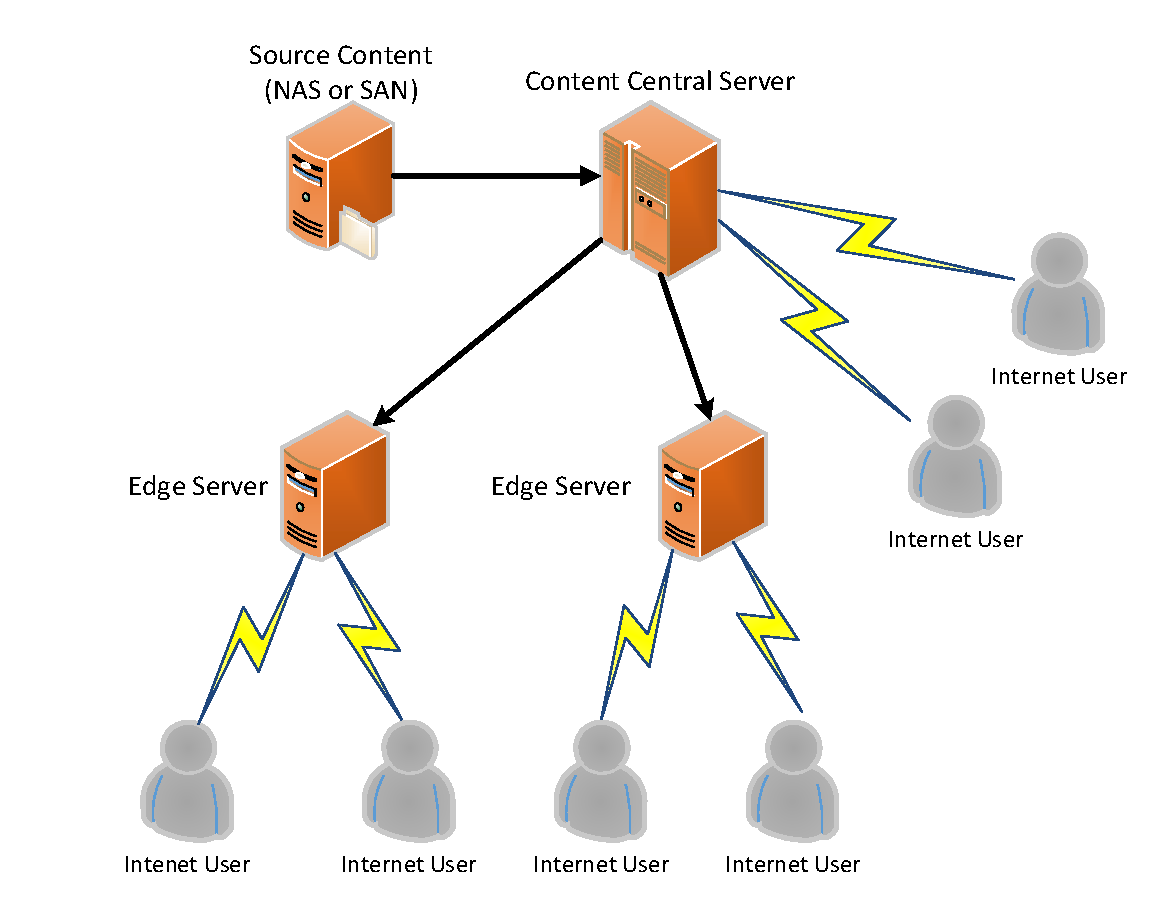
\includegraphics[width = 7cm]{cds_sample.pdf}
        \caption{An Internet content distribution system}
    \end{figure}
  \end{frame}
  
  \begin{frame}{Content Delivery}{Comparison between single content server and CDN}
    \begin{center}
    \begin{table}
    \begin{tabular}{c|cc}
      \hline
        &  Single Server & CDN \\ \hline
      throughput & low & high \\
      latency & high & low \\
      cost & high & low \\
      availability & low & high \\
      reliability & low & high \\
      update & easy & difficult \\ \hline
    \end{tabular}
    \caption{Comparison between single content server and CDN}
    \end{table}
    \end{center}
  \end{frame}

  \begin{frame}{Content Delivery}{Grid network}
    \begin{itemize}[<+->]
      \item In grid network, content is available on much more closely managed independent storage nodes.
      \item Grid network are used in peer-to-peer content delivery, where all peers are equal.
      \item All nodes in grid network are independent, but well coordinated.
      \item Grid network can make full use of existing bandwidth, and dynamically optimize the route of delivery.
    \end{itemize}
  \end{frame}

  \begin{frame}{Content Delivery}{Grid network}
    Although grid network have so many advantages, hierarchical CDN are still widely used.
    \pause
    \begin{itemize}[<+->]
      \item There exists asymmetry between servers and clients: servers send large amount of data, while clients often receive little.
      \item Not all nodes are willing to help transfer the data, nor to store the content.
      \item Grid network may face several security problems.
    \end{itemize}
  \end{frame}

  \section{Content Storage}
  \begin{frame}{Content Storage}{Storage media}
    Two types of storage media are used in content delivery system: hard disk drives and flash memory. 
    \pause
    \begin{itemize}[<+->]
      \item Hard disk drives are cheap, while flash memory is expensive;
      \item Hard disk drives have larger storage capacity than flash memory;
      \item Flash memory are much faster than hard disk drives.
    \end{itemize}
  \end{frame}

  \begin{frame}{Content Storage}{Heterogeneous storage systems}
    Because both two types of storage media have their own advantages, we can combine these two media to better the performance. This lead to the idea of heterogeneous storage.
    \pause
    \begin{itemize}
      \item NAS, SAN, or object storage system, likely uses hard disk drives, to store massive data.
      \item Central server or edge servers, may use both hard disk drives and flash memory, to accelerate the delivery of the content.
    \end{itemize}
  \end{frame}
  
  \section{Data Compression}
  \begin{frame}{Data Compression}{Definition}
    Data compression is the process to reduce the number of bits used to represent the information. Decompression is the inverse process of data compression. \par
    \pause
    Data compression can be either lossless or lossy:
    \begin{itemize}
      \item Lossless compression reduces the number of bits by eliminating statistical redundancy. It can be used for general purpose.
      \item Lossy compression reduces the number of bits by removing unnecessary or less important information. It is usually used in compressing multimedia content.
    \end{itemize}
  \end{frame}
  
  \begin{frame}{Data Compression}{Data compression in content delivery}
    Since bandwidth is expensive, data compression is very meaningful in content delivery. However, compression and decompression also take a lot of time, which may increase the latency. \par
    \pause
    Some standardized compression algorithms, such as H.264 and H.265, balance the compression rate and time cost, so they are suitable for Internet content delivery.
  \end{frame}
  
  \section{Summary}
  \begin{frame}{Summary}
    \begin{itemize}
      \item Hierarchical CDN
      \item Heterogeneous storage system
      \item Data compression
    \end{itemize}
  \end{frame}
  
  \section{}
  \begin{frame}{Q \& A}

  \end{frame}
\end{document}
